\capitolo{Modellistica di sistemi meccanici}
In seguito saranno esposti una serie di modelli utili per diversi aspetti fisici presenti nei sistemi meccanici.

\sezione{Bilancio di Potenza}
Per studiare i sistemi meccanici viene utilizzato il bilancio di potenza, per cui vi sia variazione di energia cinetica.
\[\sum_i W_i = \derivata{E_c}{t}\]
La somma delle potenze (erogate e assorbite) dalle forze esterne è uguale alla derivata nel tempo dell'energia cinetica dell'intero sistema.

\paragrafo{Potenza:}
La potenza nel caso di forza e velocità applicate in un punto di moto cartesiano è: $W_i=\pm F_i \cdot v_{i\parallel}$, dove il segno è scelto in base alla concordanza o discordanza dei segni delle convezioni\footnote{Quando si parla di convenzioni si intende una scelta arbitraria di segni che potrebbe o meno rappresentare il verso fisico della grandezza rappresentata.} dei segni di forza e velocità tangente;
Nel caso di coppia e velocità angolari applicate rispetto un asse di rotazione è: $W_i = \pm C_i \cdot \VelAng_i$, dove anche in questo caso il segno viene scelto in base alla concordanza o discordanza dei segni delle convenzioni di coppia e velocità angolare.

\paragrafo{Energia Cinetica:}
L'energia cinetica nella formula è quella totale del sistema che è pari alla sommatoria delle singole energie cinetiche.

\sottosezione{Step di convenzione}
In seguito sono esposti i passi tipici da effettuare quando si vuole scegliere una convenzione in un sistema:

\begin{enumerate}
    \item Convenzione di positività di $C_m$
    \item Convenzione di velocità degli alberi, con $\VelAng_m$ concorde a $C_m$
    \item Di conseguenza al punto 2 determinare $\VelAng_c$ in base al riduttore e in particolare se sia invertente o meno
    \item Introduzione del rapporto di trasmissione $\tau_r=\frac{\VelAng_c}{\VelAng_m}$, per cui, considerando il rapporto costante vale anche $\tau_r=\frac{\AccAng_c}{\AccAng_m}$
    \item Infine scelgo la convenzione per la coppia di carico $C_c$, che tendenzialmente sarà opposta alla convenzione di velocità $\VelAng_c$.
\end{enumerate}

\sottosezione{Motore Riduttore Carico}
Esempio classico di sistema meccatronico, in prima approssimazione valutato con idealità di riduttore (senza gioco, senza perdite di potenza, momento di inerzia nullo) e momento di inerzia del carico costante.

\begin{figure}[h]
    \centering
    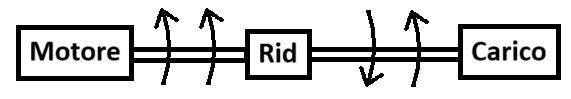
\includegraphics[width=0.4\textwidth]{Immagini/motoreriduttorecarico_id.png}
    \caption{Schema ideale}
\end{figure}


\begin{itemize}
    \item $J_c$: momento di inerzia del carico rispetto il suo asse di rotazione\footnote{NB: L'asse attorno cui viene calcolato il momento di inerzia va sempre specificato!!}
    \item $J_m$: momento di inerzia del motore rispetto il suo asse di rotazione
    \item $C_m$: coppia erogata dal motore, considerata come coppia esterna perché "applicata" dallo statore al rotore
    \item $C_c$: coppia applicata al carico.
\end{itemize}

\paragrafo{Bilancio potenza:}
La potenza delle forze esterne del sistema è data dalla potenza erogata dal motore e quella assorbita dal carico: $\sum_i W_i=C_m \VelAng_m -C_c \VelAng_c=\left(C_m -C_c \tau_r\right)\VelAng_m$. L'energia cinetica è data dalla somma delle singole energie cinetiche, quindi contributo di inerzia del motore e del carico: $E_c=\mezzo \left(J_m + J_c\tau_r^2 \right)\VelAng_m^2=\mezzo J_{eq} \VelAng_m^2$.
La derivata della energia cinetica diventa quindi $\derivata{E_c}{t}=\mezzo J_{eq}\derivata{\VelAng_m^2}{t}=J_{eq}\VelAng_m \AccAng_m$.
Considerando quindi che solitamente del carico sono note o ricavabili le specifiche, determino la coppia erogata dal motore, a seguito di semplificazioni: \[C_m=\left(J_m+J_c\tau_r^2\right)\AccAng_m+C_c\tau_r\]

\paragrafo{Trasmissioni in serie:}
Nel caso vi fossero nel sistema trasmissioni in serie quanto detto sopra sarebbe ancora valido, la differenza sostanziale si vedrebbe nel momento di inerzia equivalente.
Nel caso di un riduttore avente in serie un sistema vite madrevite, su cui è posato un carico da traslare, si otterrebbe $J_{eq}=J_m+J_v \tau^2_r + M \tau_r^2 \tau_v^2$, in questo caso inoltre il carico non sarebbe una coppia, bensì una forza: $C_m=J_{eq}\AccAng_m + F_r \tau_r \tau_v + C_a \tau_r$. \label{TrasmissioneSerie}

\begin{figure}[h]
    \centering
    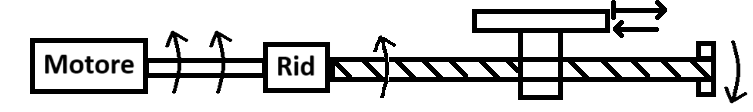
\includegraphics[width=0.5\textwidth]{Immagini/mrc_vite_madrevite.png}
    \caption{Schema trasmissioni in serie}
\end{figure}


\sottosezione{Perdite di potenza in trasmissione}
Una trasmissione reale avrà una certa perdita di potenza legata a fenomeni di attrito, che possono essere raggruppati in un unico contributo: $\sum_i W_i - W_p = \derivata{E_c}{t}$, con $W_p>0$.
Inoltre è possibile definire un rendimento: $\eta=\frac{|W_{out}|}{W_{in}}$.

\paragrafo{Fattori critici per rendimento:} 
I fattori che influenzano maggiormente il rendimento sono:
\begin{itemize}
    \item Tipo di trasmissione, quindi il tipo di geometria e di strisciamento superficiale
    \item Stato delle superfici: tipo di materiale, rugosità, lubrificazione, trattamenti superficiali, pulizia
    \item Condizioni operative come temperatura, coppia/forza/velocità trasmessa
\end{itemize}
Nonostante ciò a catalogo è tipico trovare un unico valore, tendenzialmente la condizione migliore, nominale.

\paragrafo{Verso del flusso di potenza:}
Il riduttore ha un verso preferenziale per cui il rendimento è migliore, ed è cosa comune nei casi in cui vi sia una differenza di velocità.
Per rotismi epicicloidali il rendimento migliore è quello da riduttore; per viti madreviti, quello migliore è da rotazione a traslazione.
Esiste una relazione empirica tra rendimento preferenziale e non:
\[
\eta_\textup{non preferenziale} = 
\begin{cases} 
    2 - \frac{1}{\eta_\textup{pref}} & \text{se } \eta_\textup{pref} \geqslant 0.5 \\
    0 & \text{se } \eta_\textup{pref} \leqslant 0.5
\end{cases}
\]

\sottoparagrafo{Irreversibilità:}
Rendimento nullo significa irreversibilità del moto, si parla di irreversibilità quando la potenza trasmessa ha un unica direzione possibile. Questo può essere un fenomeno voluto, es crick della macchina o vite di tenuta in una struttura, o meno.

\paragrafo{Motore Riduttore Carico, Moto Diretto:}
A differenza di quanto visto in precedenza, in questo caso la potenza che entra nel riduttore e quella che esce non è la stessa, una parte della potenza in ingresso $W_{in}$ sarà dissipata per effetti di attrito unificati all'interno di $W_p$. 
Noto che $W_p=(1-\eta_r) W_{in}$ (valida sia per moto diretto sia per moto retrogrado), considerando la potenza sia erogata dal motore il riduttore vede in ingresso una potenza $W_{in}=C_m \VelAng_m - J_m \VelAng_m \AccAng_m$, mentre la potenza di uscita dal riduttore, quindi quella che arriva al carico, è data da $W_{out}=W_{in}-W_p$, infine, a seguito di semplici passaggi, a partire dal bilancio di potenza: $C_m \VelAng_m - J_m \VelAng_m \AccAng_m - W_p^{dir} - J_c \VelAng_c \AccAng_c - C_c \VelAng_c = 0$, si ottiene la seguente espressione della coppia del motore:
\[ C_m = \left(J_m+J_c\frac{\tau^2_r}{\eta_r^{dir}}\right) \AccAng_m + C_c\frac{\tau_r}{\eta_r^{dir}} \]
In cui è chiaro come il rendimento vada a influenzare unicamente i termini a valle del riduttore, e come, essendo $0<\eta_r^{dir}<1$, vada ad aumentare la coppia che il motore deve erogare, come atteso.

\paragrafo{Motore Riduttore Carico, Moto Retrogrado:}
In modo simile al caso di moto diretto, nel moto retrogrado la potenza in ingresso al riduttore è data da $W_{in}=-C_c\VelAng_c - J_c \VelAng_c \AccAng_c$, mentre la potenza di uscita è $W_{out}=W_{in}-W_p^{retr}$, a partire dal bilancio di potenze, a seguito di manipolazioni, si ottiene la seguente espressione della coppia del motore:
\[ C_m = \left(J_m + J_c \tau_r^2\eta_r^{retr} \right)\AccAng_m + C_c\tau_r \eta_r^{retr} \]
In cui è evidente che l'attrito vada ad aiutare il motore a frenare il carico, come atteso.

\sottoparagrafo{Caso Moto Retrogrado, Riduttore Irreversibile:}
Nel caso in cui $\eta_r^{retr}=0$, l'attrito del riduttore va ad annullare il carico visto dal motore (a meno dell'inerzia del rotore stesso), si parla quindi di carico autofrenante.

\begin{figure}[h]
    \centering
    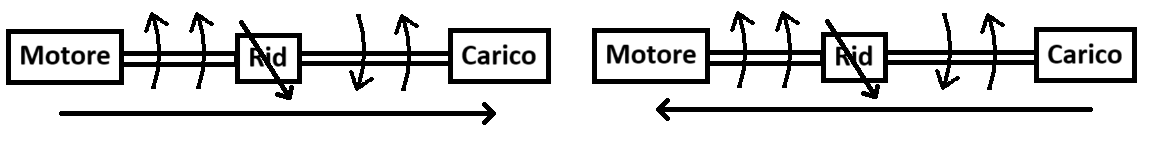
\includegraphics[width=0.7\textwidth]{Immagini/mrc_moti_diretti_vs_retrogrado.png}
    \caption{Schemi di moto diretto (sx) e retrogrado (dx)}
\end{figure}

\paragrafo{Moto Diretto vs Retrogrado:}
Per distinguere tra i due casi occorre valutare il carico, in particolare determinare se assorbe o eroga potenza:
\[
\begin{cases}
    -C_c\VelAng_c - J_c \VelAng_c \AccAng_c < 0 \text{ il carico assorbe potenza: moto diretto} \\
    -C_c\VelAng_c - J_c \VelAng_c \AccAng_c > 0 \text{ il carico eroga potenza: moto retrogrado}
\end{cases}
\]

\paragrafo{Rendimento generalizzato:}
Per semplificare l'utilizzo del rendimento negli esercizi, in cui è facile avere situazioni di continuo scambio tra modo diretto e retrogrado, è opportuno introdurre un rendimento generalizzato, che vada quindi a rappresentare i possibili casi con scrittura più compatta, evitando quindi di scrivere le stesse espressioni due volte.
Viene quindi definito:
\[
\eta_r = 
\begin{cases}
    \eta_r^d \text{ se e solo se moto diretto } -C_c\VelAng_c - J_c \VelAng_c\AccAng_c < 0 \\
    \frac{1}{\eta_r^r} \text{ se moto retrogrado o condizioni statiche } -C_c\VelAng_c - J_c \VelAng_c\AccAng_c \geqslant 0
\end{cases}
\]
Questo andrebbe utilizzato all'interno della espressione della coppia del motore come fosse rendimento di moto diretto, sostituendo l'opportuno valore in base al caso:
\[
C_m = \left(J_m+J_c\frac{\tau^2_r}{\eta_r}\right) \AccAng_m + C_c\frac{\tau_r}{\eta_r}
\]

\paragrafo{Rendimento per trasmissioni serie:}
Riprendendo il caso visto in sezione \ref{TrasmissioneSerie} pagina \pageref{TrasmissioneSerie} di riduttore con in serie un sistema vite madrevite, facendo considerazioni simili al caso a singolo stadio, considerando un bilancio di potenze in cui vengano introdotti gli effetti delle perdite per ciascuno dei riduttori, a seguito di semplici di manipolazioni si ottiene l'espressione:
\[
C_m=\left(J_m+J_v \frac{\tau^2_r}{\eta_r^d} + M \frac{\tau_r^2 \tau_v^2}{\eta_r^d \eta^d_{v-mv}}\right)\AccAng_m + F_r \frac{\tau_r \tau_v}{\eta_r^d \eta^d_{v-mv}} + C_a \frac{\tau_r}{\eta_r^d}
\]
Questa soluzione è compatibile con quanto atteso, quindi che la potenza richiesta al motore aumenti con l'aumentare dell'attrito nel riduttore in condizioni di moto diretto.
In modo del tutto simile si ottiene la coppia del motore in condizione di moto retrogrado:
\[
C_m=\left(J_m+J_v \tau^2_r\eta_r^d + M \tau_r^2 \tau_v^2\eta_r^d \eta^d_{v-mv}\right)\AccAng_m + F_r \tau_r \tau_v\eta_r^d \eta^d_{v-mv} + C_a \tau_r\eta_r^d
\]

\sezione{Attrito}
L'attrito è sempre resistente e si oppone al moto.
Un classico modello detto Coulombiano di attrito lo divide in 3 termini:
\begin{enumerate}
    \item Secco o Coulombiano: Legato ad atttrito tra superfici rugose caratterizzate da "micro-incastri". Ha due possibili regimi:
    \begin{enumerate}
        \item Statico, in assenza di moto relativo
        \item Dinamico, in presenza di moto relativo
    \end{enumerate}
    \item Viscoso
    \item Aerodinamico: Proporzionale a velocità al quadrato e a area della sezione, solitamente in impianti industriali è trascurabile, anche se ci sono applicazioni in cui va tenuto da conto.
\end{enumerate}

\sottosezione{Attrito Secco:}
Una forza normale alla superficie permette di mantenere il contatto e genera una forza parallela alla velocità e verso opposto, seguendo questa convenzione è definita la forza di attrito dinamico coulombiano: $F_{Cou}^d = N f_{Cou}^d \sign{v}$.
Il coefficiente di attrito dinamico dipende da: materiale; stato superficiale (rugosità, pulizia, lubrificazione).
Il coefficiente di attrito dinamico NON dipende da: area di contatto; velocità relativa \footnote{Ci sarà una minima dipendenza, tuttavia sarà relativamente ridotta rispetto altri fenomeni.}.

\paragrafo{Attrito Statico Coulombiano:}
A partire dalle condizioni statiche serve una forza maggiore per rompere il legame tra le superfici, quindi è corretto aspettarsi $f_{Cou}^s>f_{Cou}^d$. In questo caso la forza si "adatta" alla forza da vincere, ed è caratterizzata da un termine massimo, l'espressione rappresentativa è una disequazione: $\abs{F_{Cou}} \leqslant f_{Cou}^s N$.
La forza esterna che tende a spostare il corpo, tenuto fermo dall'attrito, inizierà a muoversi non appena $F_{ext}>\abs{F_{Cou}^s}$, momento oltre il quale l'attrito passerà dall'essere statico all'essere dinamico.

\paragrafo{Catalogo:}
Nel caso di guide a strisciamento ci si può aspettare un attrito superiore a quello necessario per guide a sfere, perché tendenzialmente l'attrito legato al rotolamento è inferiore a quello di strisciamento.
Tuttavia costruttivamente le sfere devono essere mantenute in posizione e al sicuro dalle polveri e per fare ciò è necessario utilizzare delle guarnizioni di tenuta, che aggiungono quindi una forza resistenze che a seconda del caso specifico potrebbe essere deleteria.
Nel caso di attuatori lineari a cinghia l'attrito a vuoto è legato soprattutto al precarico della cinghia stessa, questo porterà ad avere una coppia di no load derivata da un modello di attrito Coulombiano. Anche in questo caso l'utilizzo di sfere permette di ridurre l'attrito rispetto lo strisciamento.
In qualunque sia l'applicazione, tendenzialmente, aumentare la taglia\footnote{La taglia è la coppia/forza erogabile.} comporta un aumento di attrito.

\sottosezione{Attrito Viscoso}
L'attrito viscoso è legato alla viscosità del lubrificante, quindi alla resistenza di taglio, ossia allo scorrimento del fluido, ed è legato a una differenza di velocità, prendendo una convenzione con attrito viscoso di verso opposto alla velocità, si può scrivere come: $F_v=f_v \dot{x}$.
A basse velocità l'attrito viscoso è trascurabile, diventa molto rilevante ad alte velocità; il discrimante per determinare quando sia trascurabile o meno dipende dal coefficiente di attrito viscoso e dall'applicazione.

\begin{figure}[h]
    \centering
    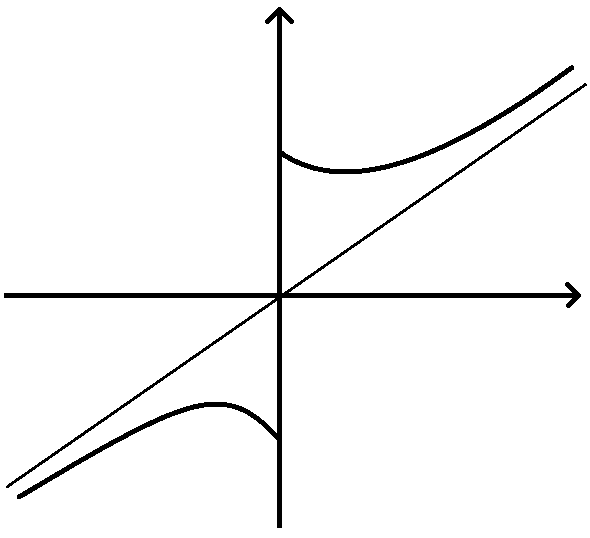
\includegraphics[width=0.3\textwidth]{Immagini/somma_effetti_attrito.png}
    \caption{Somma degli effetti di attrito}
\end{figure}